\section{Diagramas de Estados}
\label{sec:diagramaEstados}

Es esta sección se muestran los diagramas de estados y la descripción de cada uno de ellos.

\subsection{Estados de un caso de uso}

En la figura \ref{estadosCU} se muestran los estados en los que se puede encontrar un caso de uso en el sistema.

	\begin{figure}[H]
		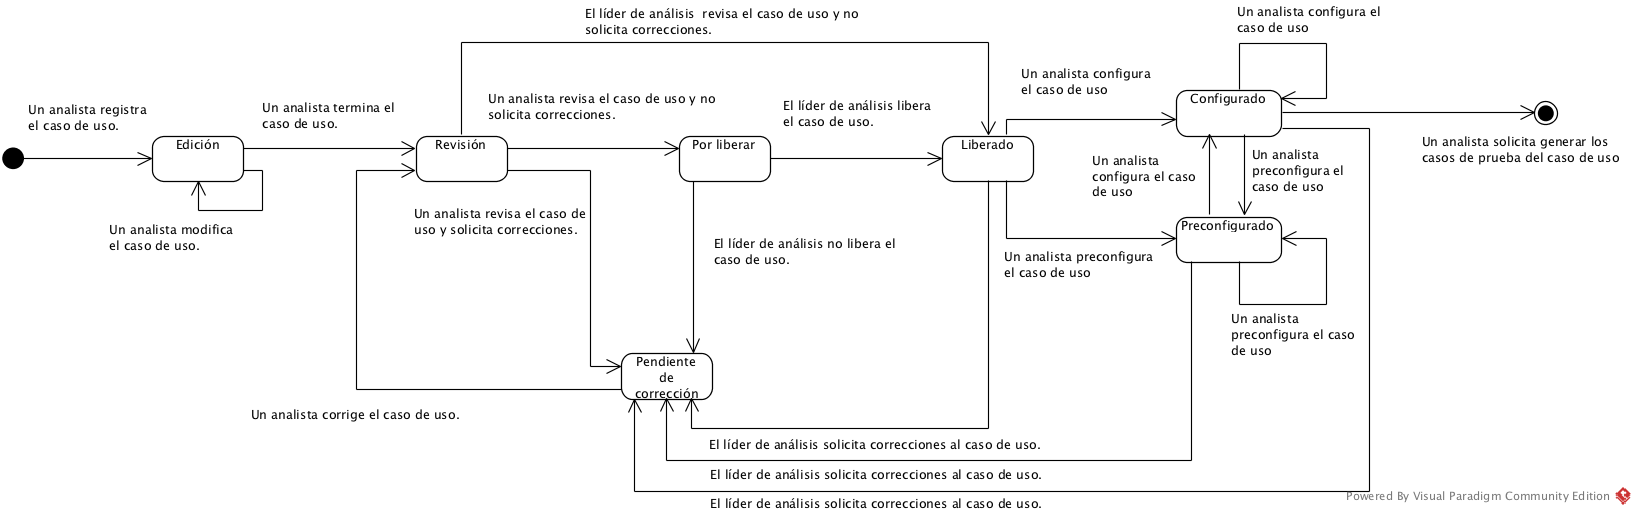
\includegraphics[scale=.45]{images/estadosCU}
		\caption{Estados de un caso de uso}
		\label{estadosCU}
	\end{figure}

	Cada estado se describe a continuación:
	\begin{itemize}
		\item \textbf{Edición}. Un caso de uso se encuentra en este estado si:
			\begin{itemize}
				\item Un analista registra el caso de uso.
				\item Un analista modifica el caso de uso.
			\end{itemize}
	\end{itemize}
	Cuando un caso de uso se encuentra en estado \textbf{Edición}, puede ser terminado o modificado.
	
	\begin{itemize}
		\item \textbf{Revisión}. Un caso de uso se encuentra en este estado si:
		\begin{itemize}
			\item Un analista termina el caso de uso.
			\item Un analista corrige el caso de uso.
		\end{itemize}
	\end{itemize}
	Cuando un caso de uso se encuentra en estado \textbf{Revisión}, puede ser revisado por algún analista e indicar si es correcto o no.
	
	\begin{itemize}
		\item \textbf{Pendiente de corrección}. Un caso de uso se encuentra en este estado si:
		\begin{itemize}
			\item Un analista revisa el caso de uso e indica que es incorrecto.
			\item El líder de análisis decide no liberar el caso de uso.
			\item El líder de análisis solicita correcciones al caso de uso.
		\end{itemize}
	\end{itemize}
	Cuando un caso de uso se encuentra en estado \textbf{Pendiente de corrección}, puede ser corregido.
	
	\begin{itemize}
		\item \textbf{Por liberar}. Un caso de uso se encuentra en este estado si:
		\begin{itemize}
			\item Un analista revisa el caso de uso e indica que es correcto.
		\end{itemize}
	\end{itemize}
	Cuando un caso de uso se encuentra en estado \textbf{Por liberar}, el líder de análisis puede decidir si es liberado o no.
	
	\begin{itemize}
		\item \textbf{Liberado}. Un caso de uso se encuentra en este estado si:
		\begin{itemize}
			\item El líder de análisis revisa el caso de uso e indica que es correcto.
			\item El líder de análisis decide liberar el caso de uso.
		\end{itemize}
	\end{itemize}
	Cuando un caso de uso se encuentra en estado \textbf{Liberado}, el líder de análisis puede solicitar correcciones al caso de uso.